\documentclass[12pt,a4paper]{article}
\usepackage[utf8]{inputenc}
\usepackage[T1]{fontenc}
\usepackage{geometry}
\usepackage{amsmath, amssymb}
\usepackage{listings}
\usepackage{xcolor}
\usepackage{booktabs}
\usepackage{array}
\usepackage{hyperref}
\usepackage{tikz}
\usetikzlibrary{shapes, arrows, positioning, trees}

\geometry{left=2.5cm, right=2.5cm, top=2.5cm, bottom=2.5cm}

\definecolor{codebg}{rgb}{0.96,0.96,0.96}
\definecolor{codegreen}{rgb}{0.0,0.5,0.0}
\definecolor{codegray}{rgb}{0.5,0.5,0.5}
\definecolor{codepurple}{rgb}{0.58,0,0.82}
\definecolor{codeblue}{rgb}{0.0,0.0,0.8}

\lstdefinestyle{javastyle}{
    backgroundcolor=\color{codebg},
    commentstyle=\color{codegreen}\itshape,
    keywordstyle=\color{codeblue}\bfseries,
    stringstyle=\color{codepurple},
    numberstyle=\tiny\color{codegray},
    basicstyle=\ttfamily\small,
    breaklines=true,
    keepspaces=true,
    numbers=left,
    numbersep=5pt,
    language=Java,
    frame=single,
    framerule=0.5pt,
    rulecolor=\color{codegray}
}

\hypersetup{colorlinks=true, linkcolor=blue, urlcolor=cyan}

\title{
    \Huge \textbf{Trees} \\[0.5em]
    \Large Binary Tree, BST \& Tree Traversals \\[0.5em]
    \large Data Structures \& Algorithms Reference
}
\author{Algorithm Study Guide}
\date{\today}

\begin{document}

\maketitle
\tableofcontents
\newpage

% ============================================================
\section{Introduction to Trees}
% ============================================================

A \textbf{tree} is a hierarchical, non-linear data structure consisting of nodes connected by edges. It is a special type of directed acyclic graph (DAG) with one designated root node.

\subsection{Key Terminology}
\begin{itemize}
    \item \textbf{Node}: Basic unit holding data.
    \item \textbf{Root}: Top-most node (no parent).
    \item \textbf{Leaf}: Node with no children.
    \item \textbf{Height}: Length of the longest path from root to a leaf.
    \item \textbf{Depth}: Distance of a node from the root.
    \item \textbf{Subtree}: A node and all its descendants.
    \item \textbf{Edge}: Connection between parent and child.
\end{itemize}

\subsection{Why Trees?}
\begin{itemize}
    \item Hierarchical data (file systems, XML/HTML).
    \item Efficient search, insert, delete: $O(\log n)$ in balanced BST.
    \item Basis for heaps, tries, AVL trees, red-black trees.
\end{itemize}

\newpage

% ============================================================
\section{Binary Tree}
% ============================================================

\subsection{Definition}
A \textbf{Binary Tree} is a tree where every node has \textbf{at most 2 children}: a \textit{left child} and a \textit{right child}. There is no ordering constraint between parent and children values.

\subsection{Properties}
\begin{itemize}
    \item Maximum nodes at level $\ell$: $2^\ell$
    \item Maximum nodes in tree of height $h$: $2^{h+1} - 1$
    \item Minimum height of $n$-node tree: $\lfloor \log_2 n \rfloor$
    \item A \textbf{full binary tree}: every node has 0 or 2 children.
    \item A \textbf{complete binary tree}: all levels filled except possibly last (filled left-to-right).
    \item A \textbf{perfect binary tree}: all internal nodes have 2 children; all leaves at same level.
\end{itemize}

\subsection{Visual Example}
\begin{center}
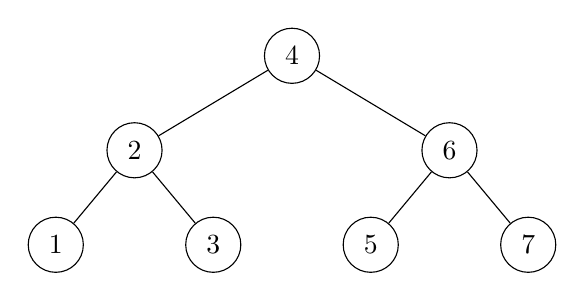
\begin{tikzpicture}[
    level distance=1.2cm,
    level 1/.style={sibling distance=4cm},
    level 2/.style={sibling distance=2cm},
    every node/.style={circle, draw, minimum size=0.7cm}
]
\node {4}
    child { node {2}
        child { node {1} }
        child { node {3} }
    }
    child { node {6}
        child { node {5} }
        child { node {7} }
    };
\end{tikzpicture}
\end{center}

\subsection{Level-Order Insertion (BFS)}
To build a complete binary tree, insert nodes level by level (left to right) using a queue. This ensures the tree remains \textit{complete} after each insertion.

\subsection{Complexity}
\begin{table}[h!]
\centering
\begin{tabular}{|l|c|c|}
\hline
\textbf{Operation}          & \textbf{Average (Balanced)} & \textbf{Worst (Skewed)} \\
\hline
Access / Search             & $O(\log n)$                 & $O(n)$                 \\
Insert (Level-order)        & $O(n)$                      & $O(n)$                 \\
Height Calculation          & $O(n)$                      & $O(n)$                 \\
\hline
\end{tabular}
\end{table}

\newpage

% ============================================================
\section{Binary Search Tree (BST)}
% ============================================================

\subsection{BST Property}
For every node $N$ in a BST:
\begin{align}
\forall x \in N.\text{left\_subtree}\colon\quad  & x < N.\text{data} \\
\forall x \in N.\text{right\_subtree}\colon\quad & x > N.\text{data}
\end{align}

This ordering property enables binary search, giving average-case $O(\log n)$ for search, insert, and delete.

\subsection{BST vs Binary Tree}
\begin{itemize}
    \item \textbf{Binary Tree}: no ordering; all BSTs are binary trees, not vice versa.
    \item \textbf{BST}: ordered; enables efficient search via divide-and-conquer.
\end{itemize}

\subsection{Insert}
\textbf{Idea}: Compare the value with the current node; go left if smaller, right if larger. Insert at the first empty spot.
\[
T(n) = O(\log n)\;\text{avg},\quad O(n)\;\text{worst (degenerate tree)}
\]

\begin{lstlisting}[style=javastyle, caption={BST Insert — Java}]
public Node insert(Node root, int data) {
    if (root == null) return new Node(data);
    if (data < root.data)      root.left  = insert(root.left, data);
    else if (data > root.data) root.right = insert(root.right, data);
    return root;
}
\end{lstlisting}

\subsection{Search}
\textbf{Idea}: At each node, compare the target with node value; go left or right accordingly.
\[
T(n) = O(\log n)\;\text{avg},\quad O(n)\;\text{worst}
\]

\begin{lstlisting}[style=javastyle, caption={BST Search — Java}]
public boolean search(Node root, int key) {
    if (root == null)        return false;
    if (root.data == key)    return true;
    if (key < root.data)     return search(root.left, key);
    return search(root.right, key);
}
\end{lstlisting}

\subsection{Delete}
Three cases arise when deleting a node:
\begin{enumerate}
    \item \textbf{No children (leaf)}: Simply remove the node.
    \item \textbf{One child}: Replace the node with its only child.
    \item \textbf{Two children}: Find the \textit{in-order successor} (smallest node in right subtree), copy its value to current node, delete the successor.
\end{enumerate}

\[
T(n) = O(\log n)\;\text{avg},\quad O(n)\;\text{worst}
\]

\subsection{BST Limitations \& Self-Balancing Trees}
A BST can degenerate into a linked list ($O(n)$) if data is inserted in sorted order. Solutions:
\begin{itemize}
    \item \textbf{AVL Tree}: Strictly balanced; rotations after each insert/delete.
    \item \textbf{Red-Black Tree}: Approximately balanced; used in Java's \texttt{TreeMap}/\texttt{TreeSet}.
\end{itemize}

\newpage

% ============================================================
\section{Tree Traversals}
% ============================================================

Tree traversal means visiting \textbf{every node exactly once} in a specific order. There are three main Depth-First traversals and one Breadth-First traversal.

\subsection{Overview}

\begin{table}[h!]
\centering
\renewcommand{\arraystretch}{1.4}
\begin{tabular}{|l|c|l|}
\hline
\textbf{Traversal} & \textbf{Order} & \textbf{Use Case} \\
\hline
In-order    & Left $\to$ Root $\to$ Right  & BST sorted output, validate BST \\
Pre-order   & Root $\to$ Left $\to$ Right  & Copy tree, serialization \\
Post-order  & Left $\to$ Right $\to$ Root  & Delete tree, expression evaluation \\
Level-order & BFS level by level           & Shortest path in tree, serialization \\
\hline
\end{tabular}
\caption{Traversal Comparison. All are $O(n)$ time, $O(h)$ space ($h$ = tree height).}
\end{table}

\subsection{In-order Traversal (L $\to$ Root $\to$ R)}

\textbf{Key Property}: For a \textbf{BST}, in-order traversal visits nodes in \textbf{ascending sorted order}.

\textbf{Example} (tree from Section 2):
\[
\text{In-order: } 1, 2, 3, 4, 5, 6, 7 \quad \leftarrow \text{sorted!}
\]

\begin{lstlisting}[style=javastyle, caption={In-order Traversal — Java}]
public static void inOrder(Node root) {
    if (root == null) return;
    inOrder(root.left);                     // LEFT
    System.out.print(root.data + " ");      // ROOT
    inOrder(root.right);                    // RIGHT
}
\end{lstlisting}

\textbf{Applications}:
\begin{itemize}
    \item Print BST elements in sorted order.
    \item Check if a binary tree is a valid BST.
    \item Generate sorted sequences from BST.
\end{itemize}

\subsection{Pre-order Traversal (Root $\to$ L $\to$ R)}

\textbf{Key Property}: Root is visited \textbf{first} before exploring children.

\textbf{Example}: $4, 2, 1, 3, 6, 5, 7$

\begin{lstlisting}[style=javastyle, caption={Pre-order Traversal — Java}]
public static void preOrder(Node root) {
    if (root == null) return;
    System.out.print(root.data + " ");      // ROOT first
    preOrder(root.left);                    // LEFT
    preOrder(root.right);                   // RIGHT
}
\end{lstlisting}

\textbf{Applications}:
\begin{itemize}
    \item \textbf{Copy/Clone} a tree structure.
    \item \textbf{Serialize} a tree (save to file; reconstruct from pre-order + in-order).
    \item Print directory/file hierarchy (parent before children).
\end{itemize}

\subsection{Post-order Traversal (L $\to$ R $\to$ Root)}

\textbf{Key Property}: Root is visited \textbf{last} after both subtrees are processed.

\textbf{Example}: $1, 3, 2, 5, 7, 6, 4$

\begin{lstlisting}[style=javastyle, caption={Post-order Traversal — Java}]
public static void postOrder(Node root) {
    if (root == null) return;
    postOrder(root.left);                   // LEFT
    postOrder(root.right);                  // RIGHT
    System.out.print(root.data + " ");      // ROOT last
}
\end{lstlisting}

\textbf{Applications}:
\begin{itemize}
    \item \textbf{Delete} a tree (children freed before parent — avoids dangling references).
    \item \textbf{Evaluate} expression trees (operands evaluated before operator).
    \item Calculate directory sizes (files computed before containing folder).
\end{itemize}

\newpage

% ============================================================
\section{Complexity Summary}
% ============================================================

\begin{table}[h!]
\centering
\renewcommand{\arraystretch}{1.5}
\begin{tabular}{|l|c|c|c|}
\hline
\textbf{Operation}     & \textbf{Avg (Balanced)} & \textbf{Worst (Skewed)} & \textbf{Space} \\
\hline
BST Insert             & $O(\log n)$              & $O(n)$                  & $O(\log n)$    \\
BST Search             & $O(\log n)$              & $O(n)$                  & $O(\log n)$    \\
BST Delete             & $O(\log n)$              & $O(n)$                  & $O(\log n)$    \\
In/Pre/Post-order      & $O(n)$                   & $O(n)$                  & $O(h)$         \\
Height of tree         & $O(n)$                   & $O(n)$                  & $O(h)$         \\
\hline
\end{tabular}
\caption{$h$ = height of tree, $n$ = number of nodes}
\end{table}

\section{Key Formulas}

\begin{align}
\text{Height of balanced BST with } n \text{ nodes:}\quad & h = \lfloor \log_2 n \rfloor \\
\text{Max nodes at level } \ell:\quad                       & 2^\ell \\
\text{Total nodes in perfect binary tree of height } h:\;  & 2^{h+1} - 1 \\
\text{In-order of BST produces sorted sequence.}
\end{align}

\end{document}
